\documentclass[UTF8]{ctexart}
\usepackage{ctex}
\usepackage{amsthm,amsmath,amssymb}
\usepackage{color}
\usepackage[colorlinks,linkcolor=red]{hyperref}
\usepackage{mathrsfs}
\usepackage{boondox-cal}
\usepackage{braket}
\usepackage{graphicx}
\usepackage{epstopdf}
\usepackage{dutchcal}
\usepackage{lmodern}
\newcommand{\rank}{\mathrm{rank}}

%.% %.% %.% %.% %.% %.% %.% %.% %.% %.% %.% %.% %.% %.%
% \begin{figure}[htbp]
%     \centering
%     \subfigure{
%     \includegraphics[height=4cm, width=6cm]{setn.eps}
%     }
% 	\;
%     \subfigure{
%     \includegraphics[height=4cm, width=6cm]{setm.eps}
%     }
% \end{figure}
% %.% %.% %.% %.% %.% %.% %.% %.% %.% %.% %.% %.% %.% %



\title{Chap 4}
\author{}
\date{}
\pagestyle{plain}
\begin{document}
	\maketitle
    \section*{4 数据分析过程}
    \subsection*{数据准备}
    首先我们应当注意到, 我们有 \href{run:../data/COVID19/country.csv}{country.csv} 以及 \href{run:../data/COVID19/daily\_info.csv}{daily\_info.csv} 两个数据文件. 而新冠疫情, 人们所最为关心的一点, 总是后来一天的新增病例. 为了实现这个目标, 我们应当尽可能地利用上已有的信息. \href{run:../data/COVID19/country.csv}{country.csv} 给我们提供了各个国家的特定信息, 我们首先就应当提取其中重要的部分.

    注意到主成分分析能够帮助我们实现上述的要求. 我们将读取数据, 处理缺失值, PCA, 并使用 k-means 进行聚类集成在 \href{run:../src/Divide\_types.m}{Divide\_types.m} 中. 此处可以调整的参数为 PCA 后截断的参数以及分类的总类数. 这里我们选取 PCA 后的前三项性质将所有 \href{run:../data/COVID19/daily\_info.csv}{daily\_info.csv} 中出现过的国家分为六类. 具体的分类可以参见 \href{run:../Project.mlx}{Project.mlx}.

    接下来我们应当考虑我们将使用什么数据进行预测. 这里首先我们会用到上面截断出的参数. 再考虑到总体的病例以及预测日期之前几天的新增病例数对预测有重要作用, 我们再加上 total\_cases 以及预测日之前四天的新增病例数作为 features. 这里我们把数据整合起来的功能集成于 \href{run:../src/Data\_Prepatraion.m}{Data\_Prepatraion.m} 中. 这里接受输入参数为希望读取的国家, 以及是否光滑化数据.

    \subsection*{预测方法的选择}
    注意到在本次作业中, 并没有无症状携带者, 易感人群, 死亡病例等数据, 所以这里传统的 SEIR 或者 SEIRS 模型并不适用. 而新增病例是与时间有很强关系的数据, 我们选择 RNN 来进行预测是自然的. 这里我们选择 RNN 中的特殊种类——LSTM 进行预测. 为方便起见, 也与 MATLAB 的风格相符, 我们直接列出网络结构:
	\begin{align*}
		&\text{sequenceInputLayer(8)} \rightarrow \\
    	&\text{fullyConnectedLayer(30)} \rightarrow \\
    	&\text{reluLayer} \rightarrow \\
    	&\text{lstmLayer(400)} \rightarrow \\
    	&\text{reluLayer} \rightarrow \\
    	&\text{fullyConnectedLayer(30)} \rightarrow \\
    	&\text{reluLayer} \rightarrow \\
    	&\text{fullyConnectedLayer(numResponses)} \rightarrow \\
    	&\text{regressionLayer}
	\end{align*}
	注意到我们的数据集并不大, 这里搭建的网络也比较小, 这使得在个人电脑上进行训练成为可能.
    \subsection*{网络训练}
    首先, 我们从不同的类别中挑出几个有代表性的国家, 这里我们的选取是 Ethiopia, Zimbabwe, Hungary, South Korea, Egypt, Australia, Canada, Iceland. 我们选取 Adam 优化器, 对上述数据训练 2000 个 epoches. 初始的学习率设置为 $0.001$, 并每 75 个 epoch 乘以 $0.95$. 定义一个 Kernel
	\[
	\mathcal{K} =
	\begin{bmatrix}
		\displaystyle\frac{1}{4}&\displaystyle\frac{1}{4}&\displaystyle\frac{1}{4}&\displaystyle\frac{1}{4}
	\end{bmatrix},
	\]
	我们将每日新增病例数与上面的核进行卷积, 考虑是两方面的: 一是为了方便网络的训练, 二是用四天的数据的平均来代替某一天的数据.
	\begin{figure}[htbp]
	    \centering
	    \subfigure{
	    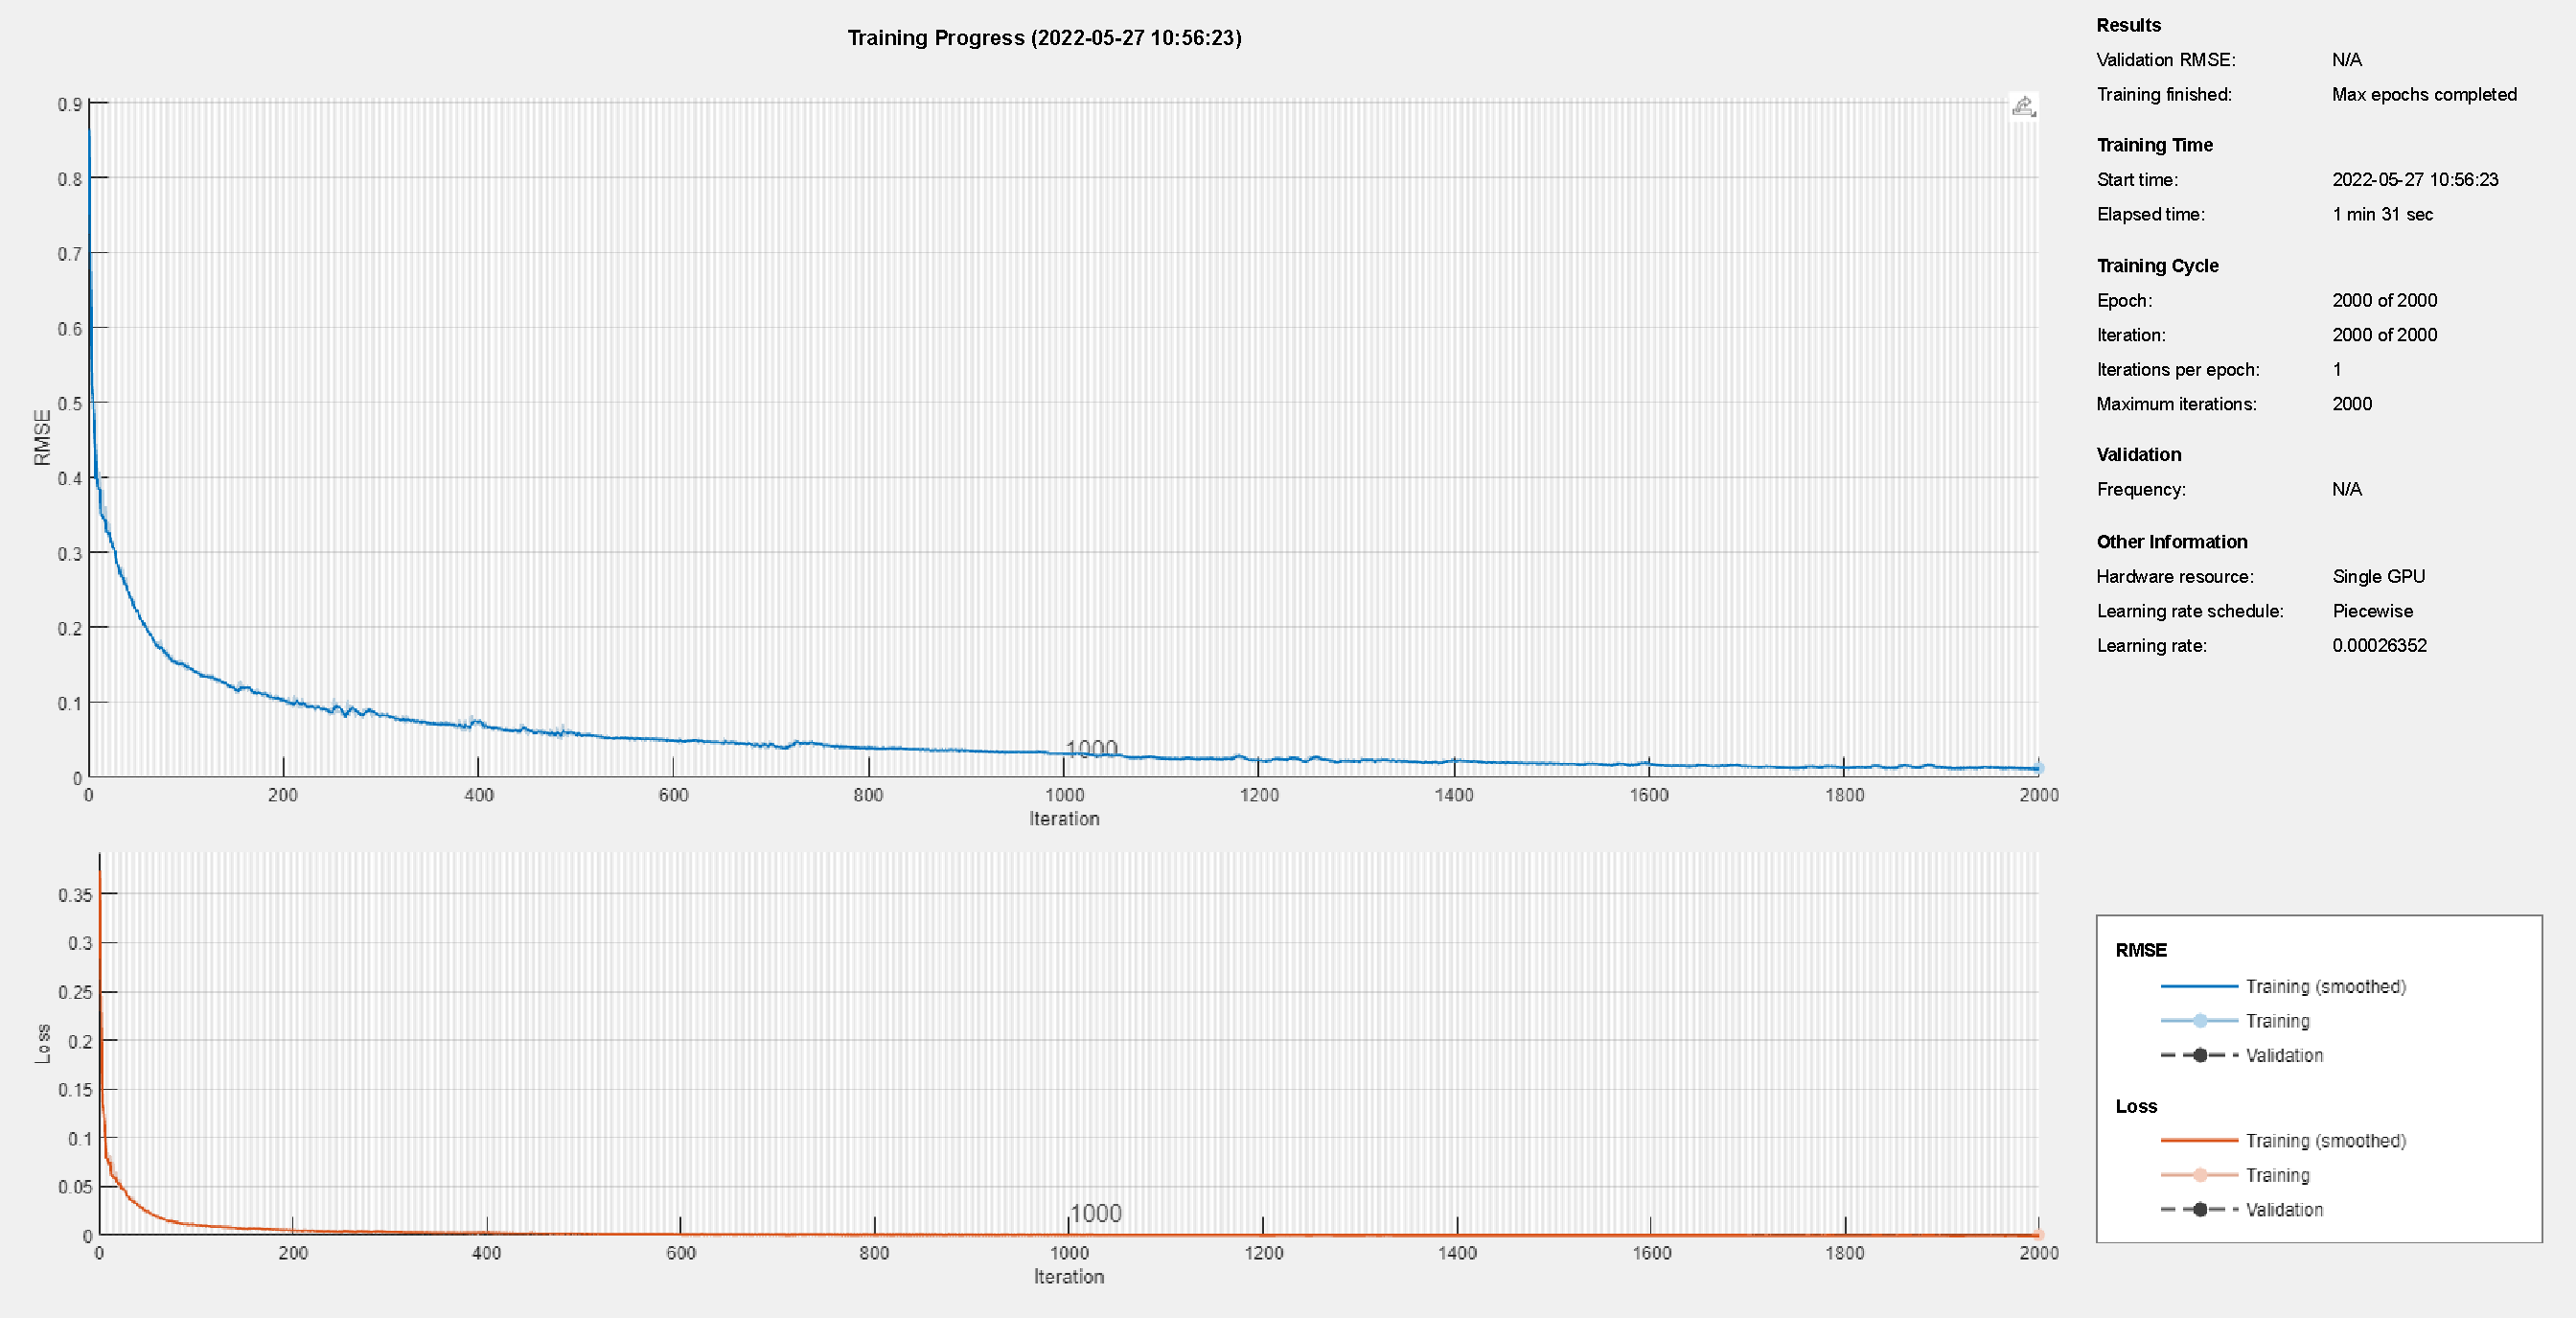
\includegraphics[height=8cm, width=12cm]{trainingprocess.pdf}
	    }
	\end{figure}
	\subsection*{结果预测}
	我们将得到的网络用于预测中国的新增病例数. 可以看到效果是很好的.
	\begin{figure}[htbp]
	    \centering
	    \subfigure{
	    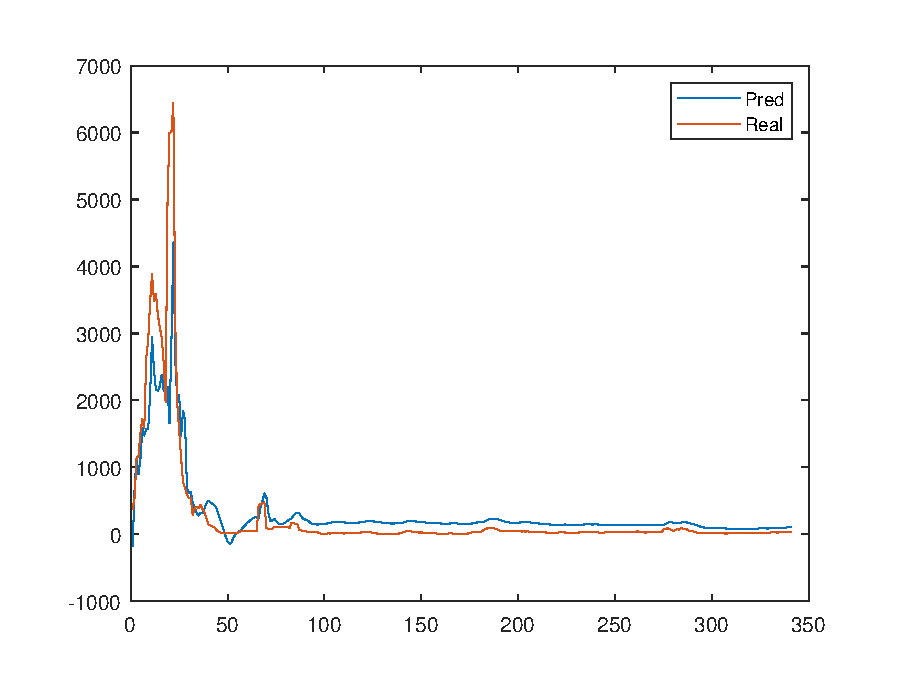
\includegraphics[height=8cm, width=12cm]{China_Pred.eps}
	    }
	\end{figure}
\end{document}
